\documentclass{beamer}
\usetheme{Singapore}
\usepackage{caption}
\usepackage{tikz}
\usetikzlibrary{shapes,arrows}
%%%%%%%% New flow
% Old Flow Define block styles
\tikzstyle{decision} = [diamond, draw, fill=blue!20, text editas=25em, text badly centered, node distance=3cm, inner sep=0pt]
\tikzstyle{block} = [rectangle, draw, fill=blue!20, text width=15em, text centered, rounded corners, minimum height=3em]
\tikzstyle{line} = [draw, -latex']
\usepackage{graphicx}
%%%%%%%%%%%%%%%%%%%%%%%%%%%%%%%%%%%%%%%%%%%%%%%%%%%%%%%%%%%%%%%%%%%%%
\title{Protein Modeling, Lecture I}
\subtitle{\textcolor{cyan}{\small LatEx, RCSB, VMD, Reduce, git, github, Entropy Maxima, CHARMM}}
\author{Noel Carrascal}
\date{August 9, 2017}
\begin{document}
\maketitle
%%%%%%%%%%%%%%%%%%%%%%%%%%%%%%%%%%%%%%%%%%%%%%%%%%%%%%%%%%%%%%%%%%%
\begin{frame}{Outline}
   \begin{enumerate}
      \item Introduction
      \item Learn about the Protein Databank at rcsb.org
      \item Download and install VMD. View Protein in VMD and learn some basic commands.
      \item How Crystal structures are obtained. Hydroge can go unnoticed, need to be added.
      \item Quick intoor to git and github. Fork and pull EntropyMaxima and CCL\_Lectures repositories.
      \item Bash shell. Intro and simple use for automating multiple step procedures.
      \item Prepare a protein structure.
   \end{enumerate}
\end{frame}
%%%%%%%%%%%%%%%%%%%%%%%%%%%%%%%%%%%%%%%%%%%%%%%%%%%%%%%%%%%%%%%%%%%
\begin{frame}{Introduction}
  \begin{columns}
      \begin{column}{0.5\textwidth}
        \begin{figure}
           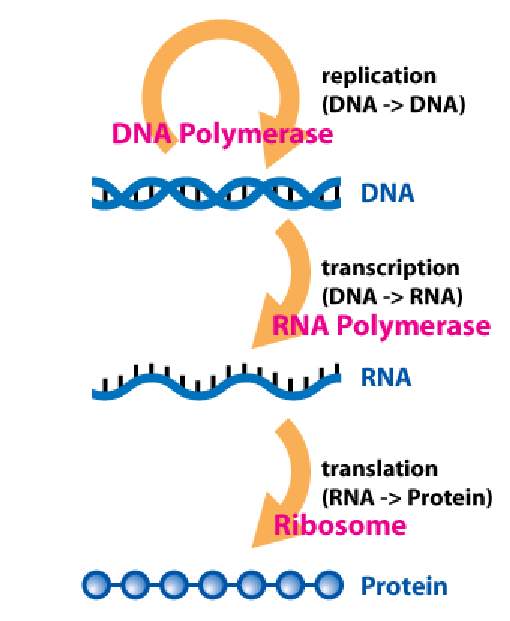
\includegraphics[width=1.4in]{/home/noel/Pictures/Presentations/Insulin/Extended_Central_Dogma_with_Enzymes}
        \end{figure}
      \end{column}
      \begin{column}{0.5\textwidth}
        \begin{figure}
           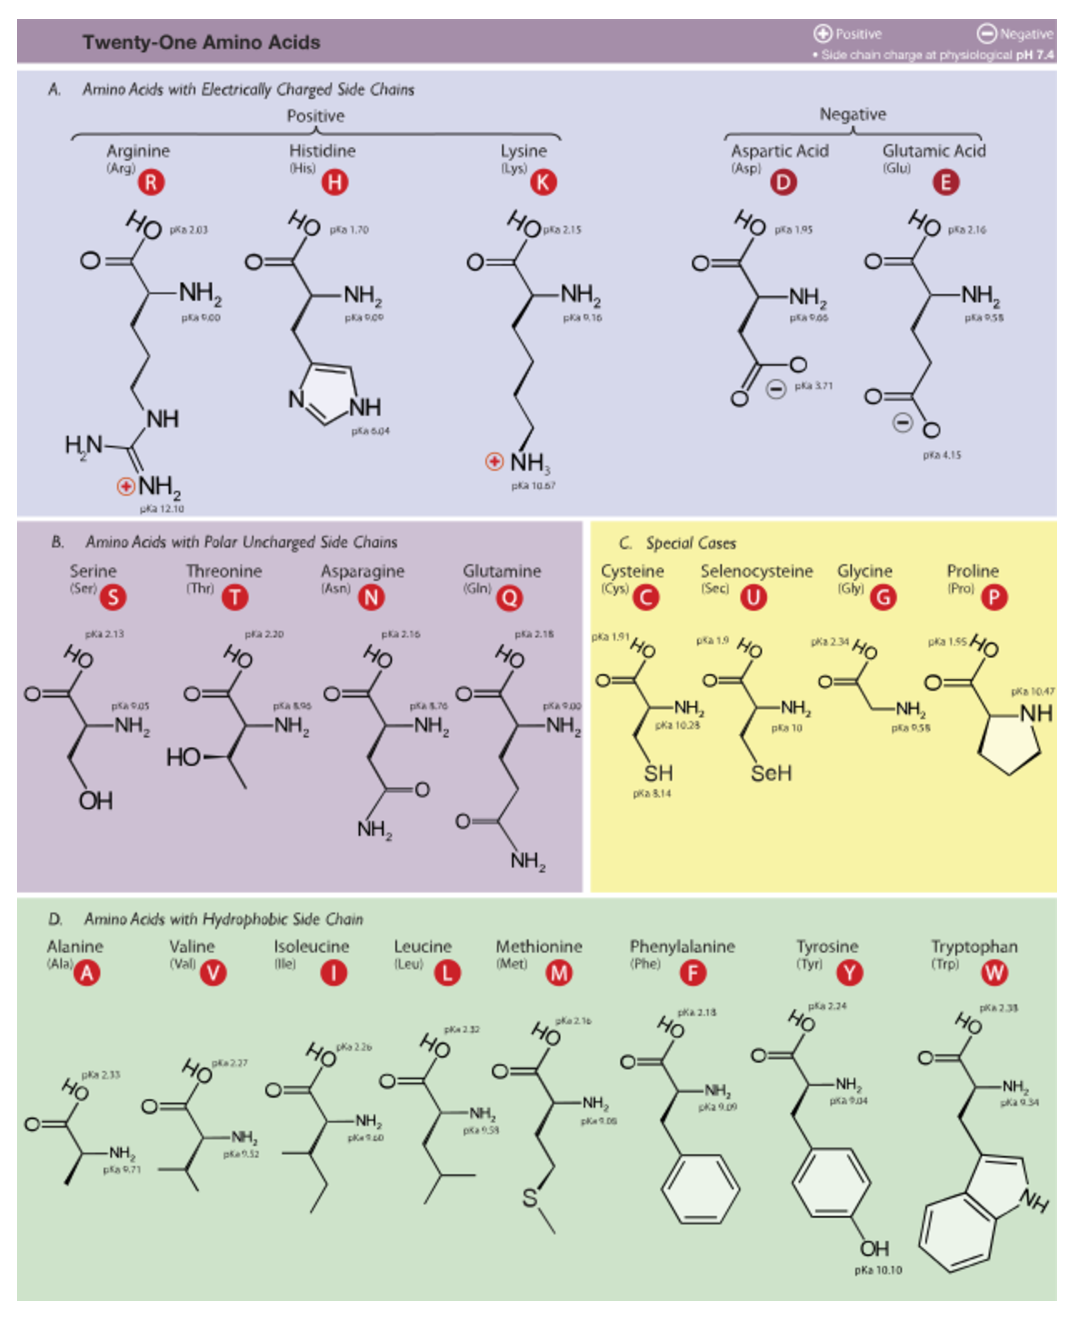
\includegraphics[width=1.4in]{/home/noel/Pictures/Presentations/Insulin/Amino_Acids}
        \end{figure}
      \end{column}
   \end{columns}
   {\tiny Licensed under CC BY-SA 3.0 via Commons https://commons.wikimedia.org/wiki/File:Extended\_Central\_Dogma\_with\_Enzymes.jpg}
\end{frame}
%%%%%%%%%%%%%%%%%%%%%%%%%%%%%%%%%%%%%%%%%%%%%%%%%%%%%%%%%%%%%%%%%%%
\begin{frame}{Protein Data Bank (www.rcsb.org)}
          \begin{center}
          \begin{figure}
           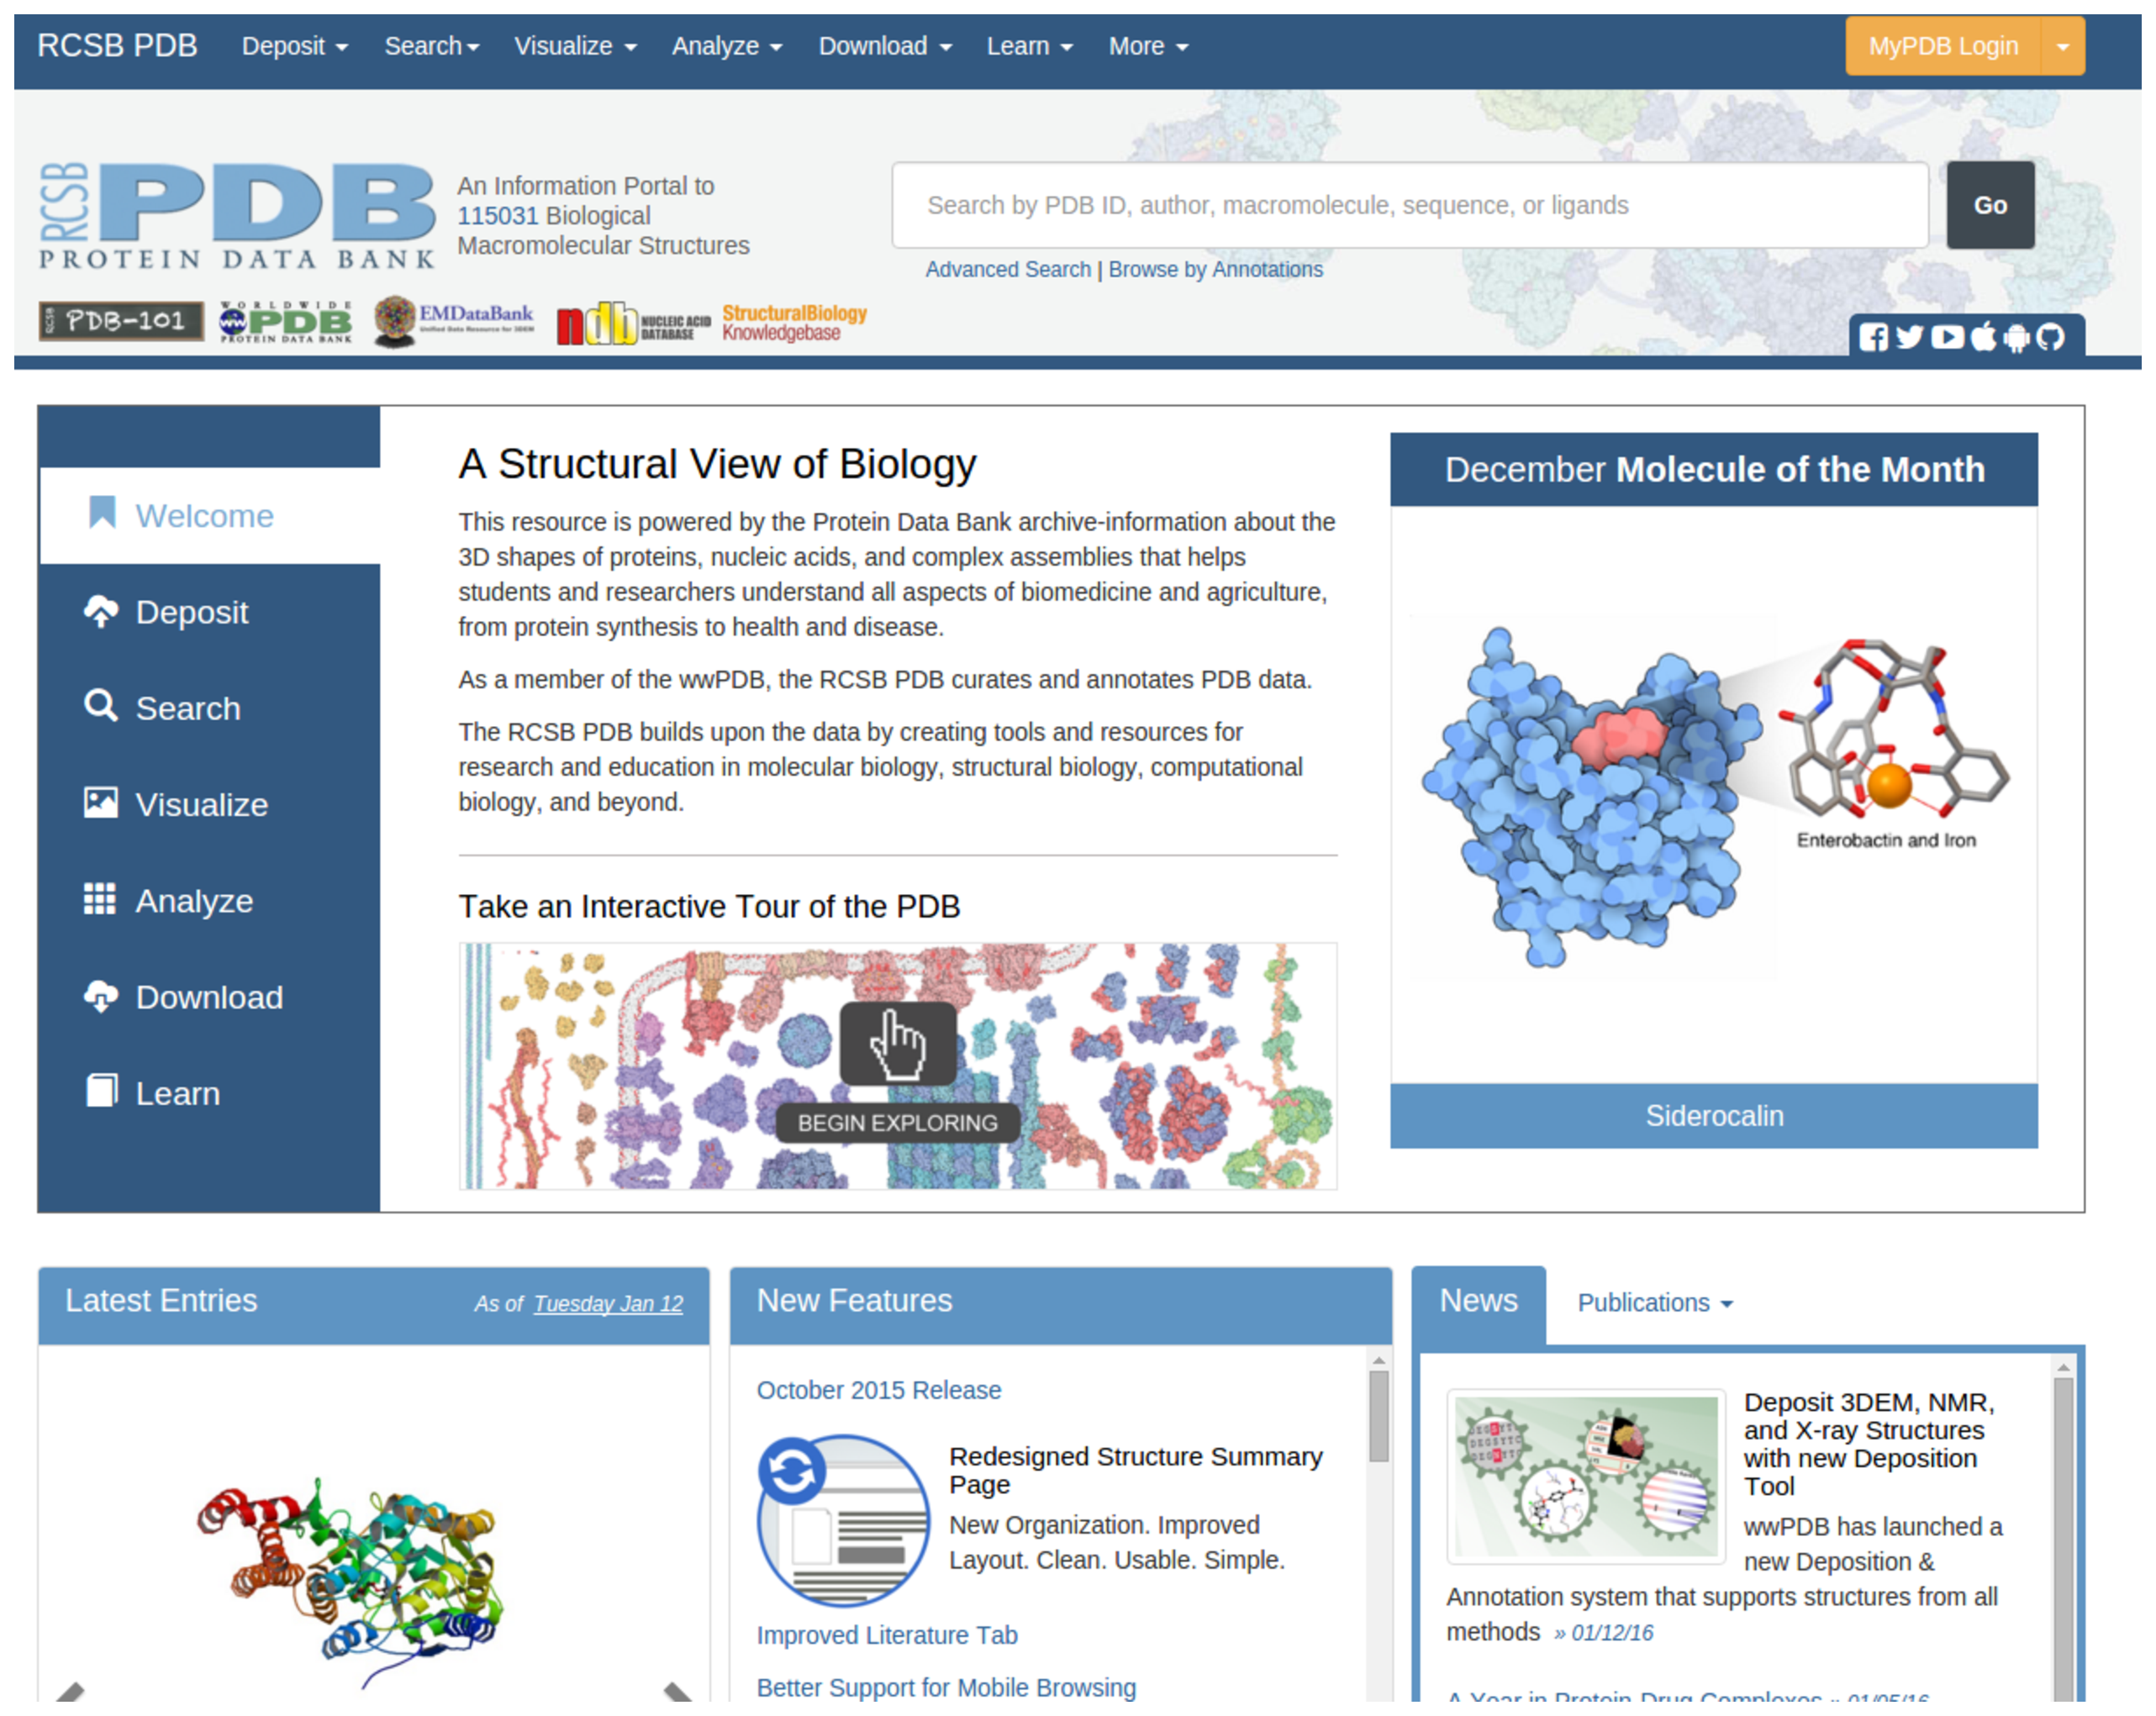
\includegraphics[width=2.1in]{/home/noel/Pictures/Presentations/Insulin/RCSB_screen_Shot}
           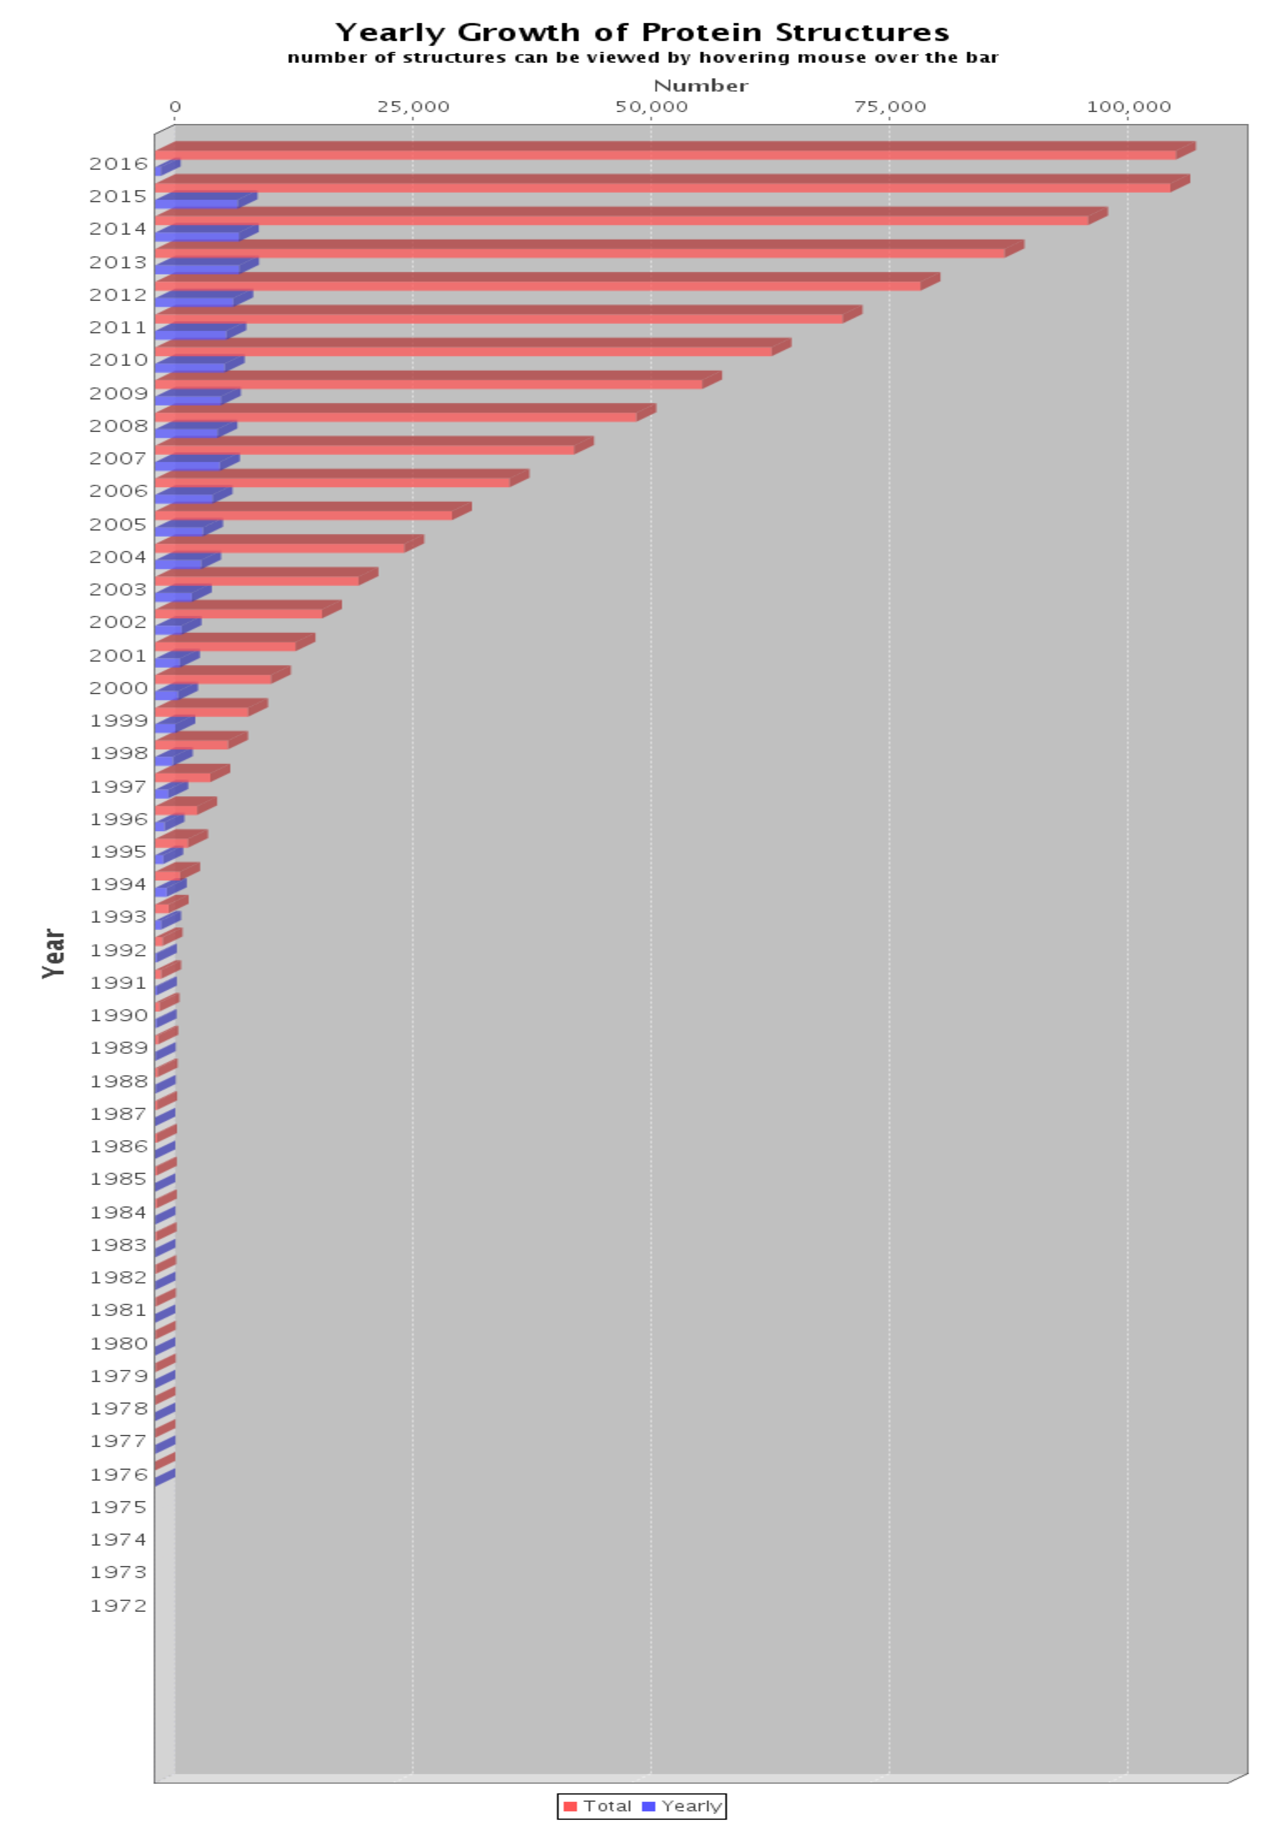
\includegraphics[width=1.2in]{/home/noel/Pictures/Presentations/Insulin/protein_structures}
          \end{figure}
          \textcolor{cyan}{\small PDB Holdings Breakdown up to 2016}
          {\tiny
          \begin{tabular}{| c | c | c | c | c | c | } \hline
               Exp.Method & Proteins & Nucleic Acids & Protein/NA Complexes & Other & Total \\
               \hline
               X-Ray & 96036 & 1698 & 4850 & 4 & 102508 \\
               NMR & 9854 & 1136 & 231 & 8 & 11229 \\
               Electron Density & 673 & 29 & 230 & 0 & 932 \\
               Hybrid & 83 & 3 & 2 & 1 & 89 \\
               Other & 170 & 4 & 6 & 13 & 193 \\
               Total & 106816 & 2870 & 5319 & 26 & 115031 \\
              \hline
          \end{tabular}
          }
          \end{center}
\end{frame}
%%%%%%%%%%%%%%%%%%%%%%%%%%%%%%%%%%%%%%%%%%%%%%%%%%%%%%%%%%%%%%%%%%%
\begin{frame}{Visualization with VMD}
  \begin{figure}
    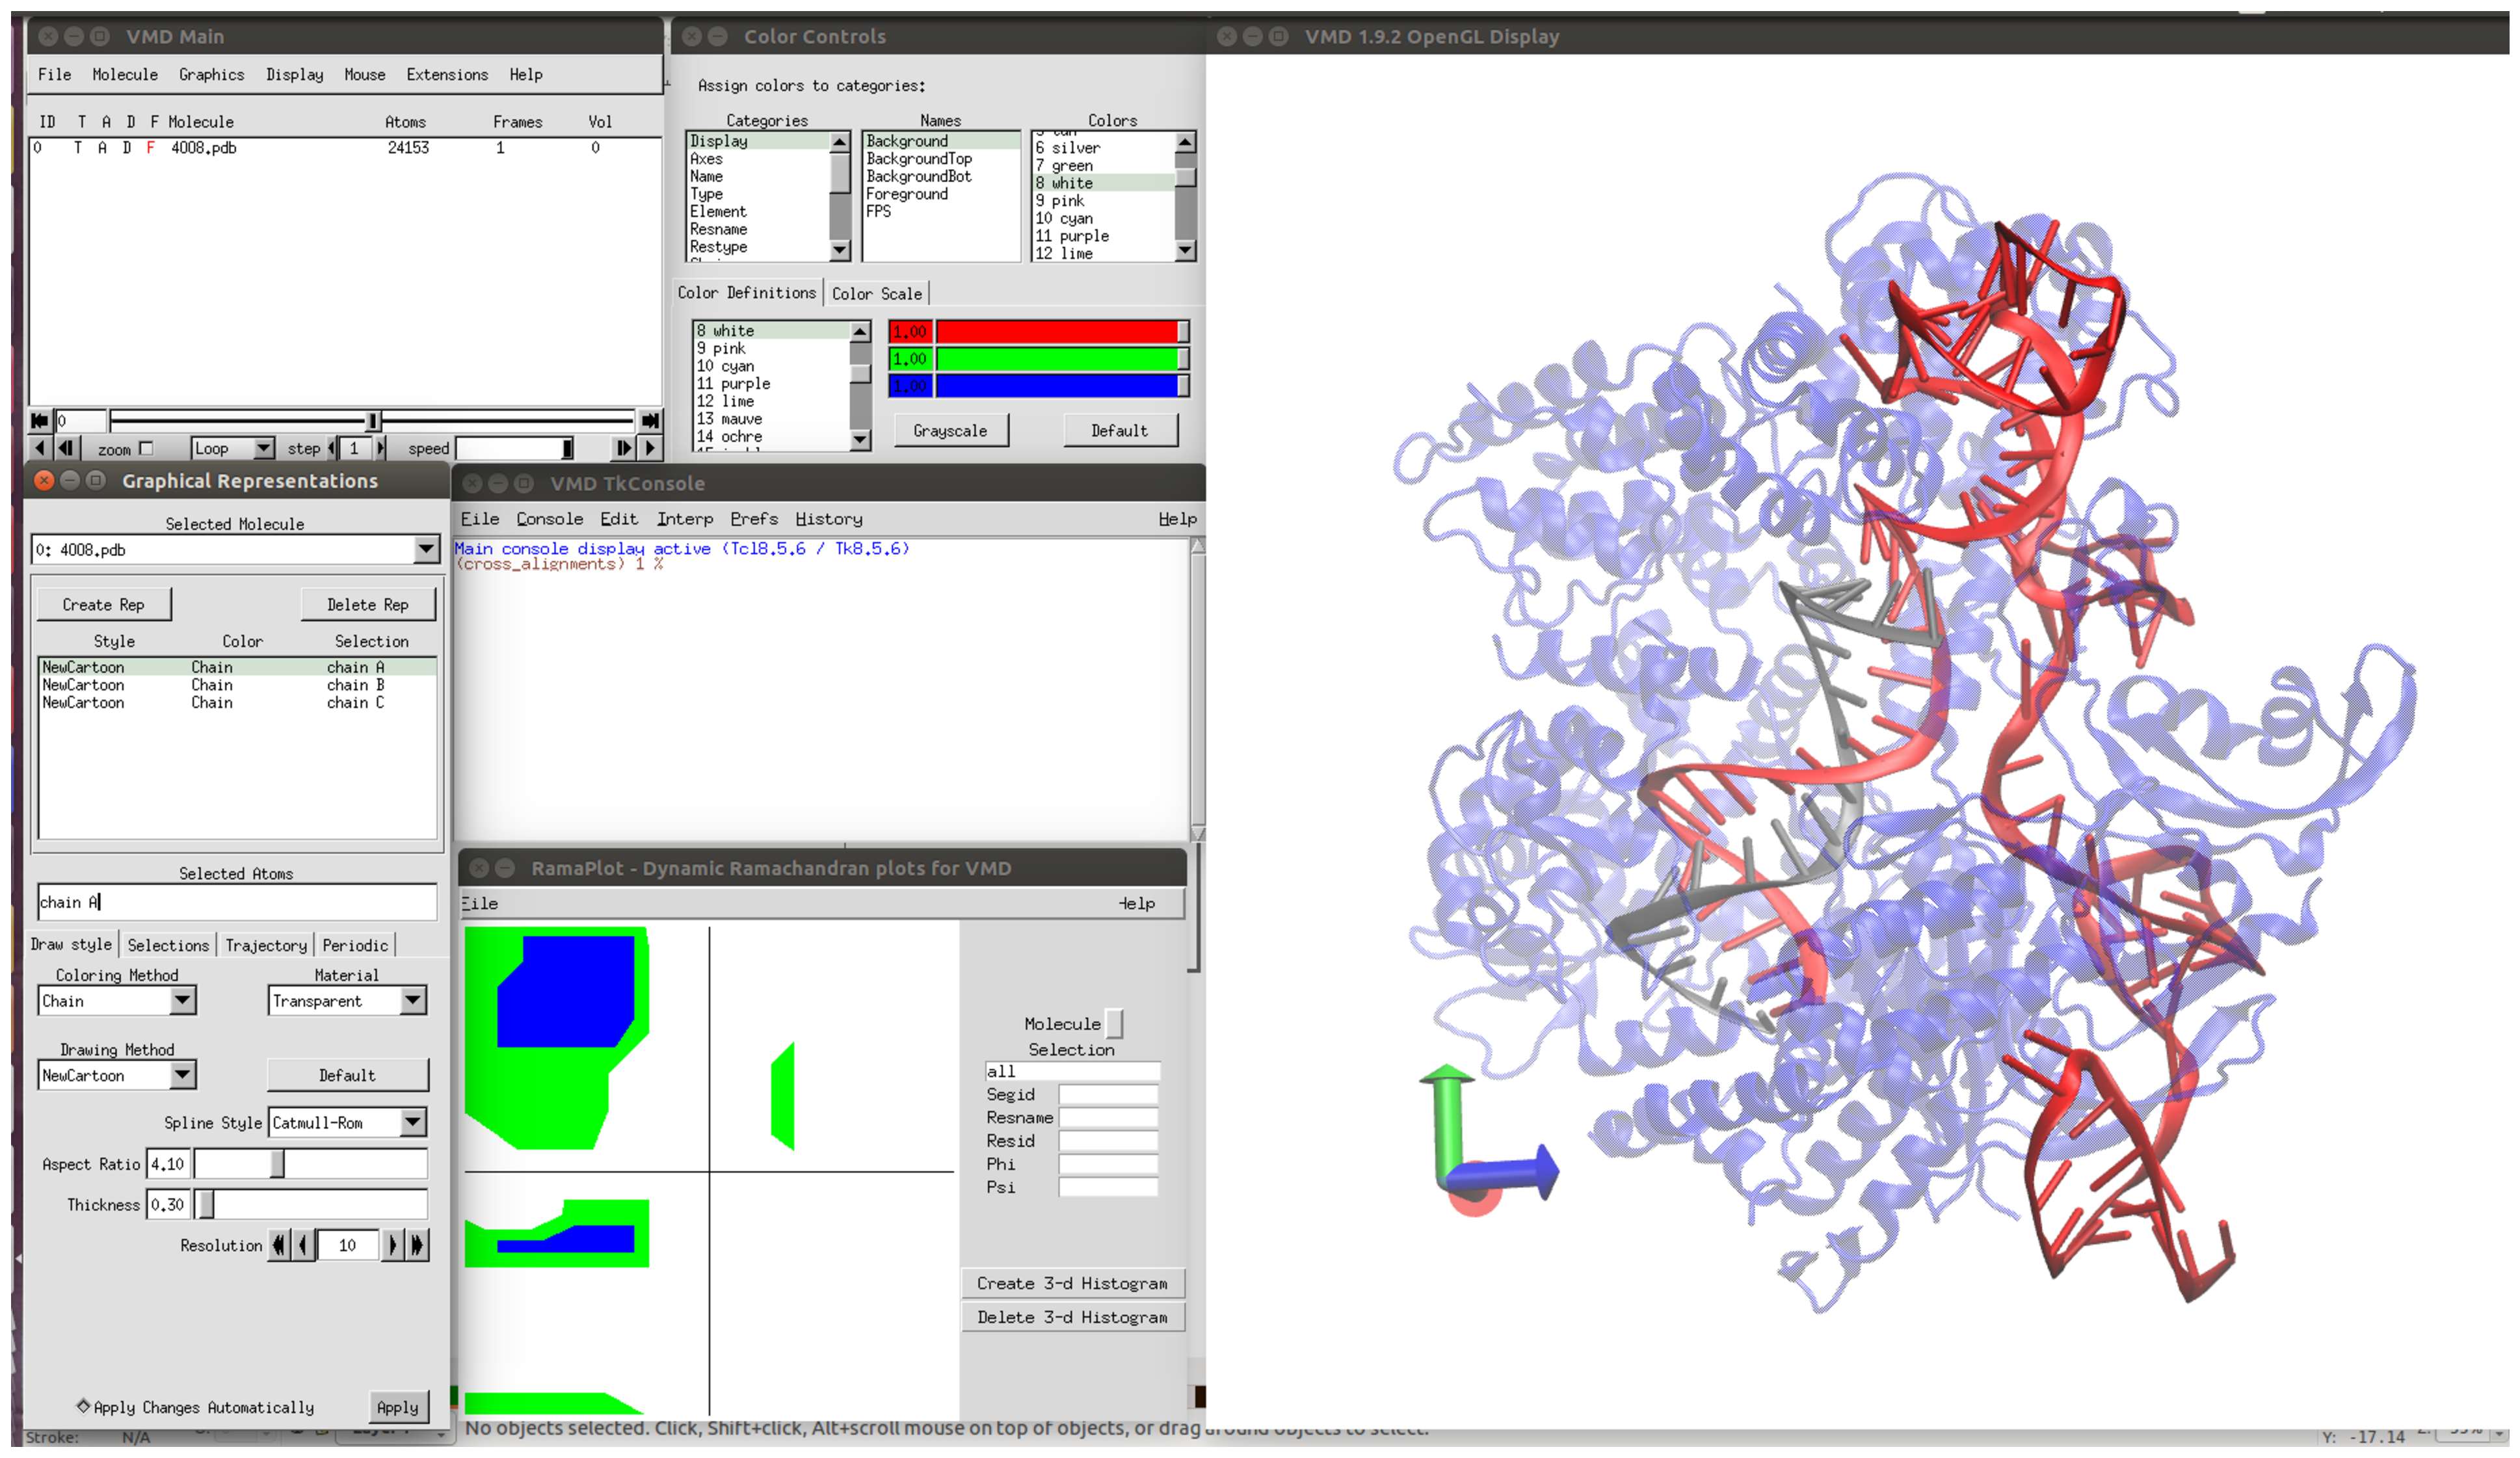
\includegraphics[width=4.3in]{/home/noel/Pictures/Presentations/Insulin/VMD}
  \end{figure}
\end{frame}
%%%%%%%%%%%%%%%%%%%%%%%%%%%%%%%%%%%%%%%%%%%%%%%%%%%%%%%%%%%%%%%%%%%
\begin{frame}[shrink=30]{Using VMD I: Loading and Viewing files.}
   \begin{enumerate}
      \item Download, install and open VMD from http://www.ks.uiuc.edu/Research/vmd/
      \item Two windows open when VDM is launched. They are labeled 'VMD Main' and 'VMD 1.9.3 OpenGL Display'.
      \item Download the protein structures 2hiu.pdb (insulin) from www.rcsb.org.
      \item To Open 2hiu, in the 'VMD main' window go to the menu option File $>$ New Molecule...
      \item A window opens with three fields, make sure those fields have the right entries:
            \begin{enumerate}
               \item In the "Load Files For:" Pull down menu, select "New Molecule"
               \item Click the "Browse" button to find the PDB file you want to open (Insulin or 2hiu)
               \item The "Determine File Type" field usually detects the right format for the file to upload, but be sure
                     it is PDB in this case. Some structural file formats have the the same file name extension for different formats
                     and VMD might pick the wrong one (e.g. The crd file name extension is used for both Amber and CHARMM).
               \item Click the "Load" button.
            \end{enumerate}
      \item On the Display windows, the mouse pointer is an arrow. Hold down the right button in your mouse and move it. It rotates.
      \item Hit the 'T' (pointer becomes a hand) letter in the keyboard and holding down the right button of the mouse translates the molecule. 
            Hit the 'R' key to go back to rotate pointer is again an arrow.
      \item Hit 'Ctrl A' or 'Ctrl Z' to zoom in and out respectively.
      \item Hit 'Y' and the protein rotates by itself. Click anywhere in the display and move pointer while holding right button in the mouse to stop the rotation.
            Rotation, translation and zoom are possible while the protein rotates.
      \item In the 'VMD main' window go to Display $>$ Reset View to bring back the protein to the original position right after loading.
   \end{enumerate}
\end{frame}
%%%%%%%%%%%%%%%%%%%%%%%%%%%%%%%%%%%%%%%%%%%%%%%%%%%%%%%%%%%%%%%%%%
\begin{frame}[shrink=10]{Using VMD II: Labels and Measurements.}
   \begin{enumerate}
      \item In the 'VMD Main" window go to menu option Graphics $>$ Labels...
      \begin{enumerate}
          \item Hit '1' on the keyboard, and the pointer in the display changes from an arrow to a cross. Click on an atom in the Display. 
            You will see information about that atom both on the display and Labels window. Click again on the atom, what happens on the display
            and Label Window?
          \item Hit '2' on the key, the pointer is still a cross but this time it does something different. Click on one atom, and then click on 
                a second atom. The distance appears on the Display. On the Labels Window, pull the drop down menu and go to bonds. What do you see?
          \item Hit '3', still a cross, click on three atoms, and drop down menu to Angles. 
          \item Hit '4', still a cross, click on Four atoms, and drop down menu to Dihedrals.
      \end{enumerate}
      \item Hit 'R' to avoid making an involuntary selection for measurement. The pointer goes from a cross back to an arrow. 
   \end{enumerate}
\end{frame}
%%%%%%%%%%%%%%%%%%%%%%%%%%%%%%%%%%%%%%%%%%%%%%%%%%%%%%%%%%%%%%%%%%
\begin{frame}[shrink=15]{Using VMD III: Graphic Representations and save a visualization states.}
   \begin{enumerate}
      \item In the 'VMD Main" window go to menu option Graphics $>$ Representations...
      \item The default Style, Color and selection is Lines, Name and All. Lets Play with the Coloring Method and Drawing Method
            Using the pull down menus in the 'Draw Style' tab below.
      \item The 'Selected Atoms' Field is not obvious to understand. Go to the 'Selections' tab' For some options. I will go over a few only.
      \begin{enumerate}
          \item Double click 'backbone', hit space, click the 'and' button, hit space, double click 'type', space, and double click CA. Hit 'Apply',
                and watch the display. If your selection is wrong you will get a message. If the selection is an empty set, you will see nothing.(of course).
                Play with other combination of selections.
          \item 'resid 1', 'resid 1 and chain A', 'resid 1 to 10 and chain A'. Substitute 'resid 1' with 'resname CYS'.
          \item An useful one, not easy to figure out: 'all (within 5 of resid 1 and chain A)'.
      \end{enumerate}
      \item You could spend a long time working on graphic representation. It is possible to save this visualization stat.
            Go to File $>$ Save Visualization State, pick a name and directory. To reload, File $>$ Load Visualization State.
      \item VMD can do a lot more. Reading its manual or doing Google searches can give you more options. 
   \end{enumerate}
\end{frame}
%%%%%%%%%%%%%%%%%%%%%%%%%%%%%%%%%%%%%%%%%%%%%%%%%%%%%%%%%%%%%%%%%%%
\begin{frame}[shrink=30]{X-Ray Crystallography and its Limitations}
       \begin{enumerate}
             \item Hydrogen atoms have an electron density that X-rays might not detect, so they might not show up in crystal structures.
             \item Regions of the protein with high thermal motion at cryogenic temperatures will not diffract x-rays in a way that can resolve their coordinates.
       \end{enumerate}
  \begin{columns}
      \begin{column}{0.5\textwidth}
        \begin{figure}
           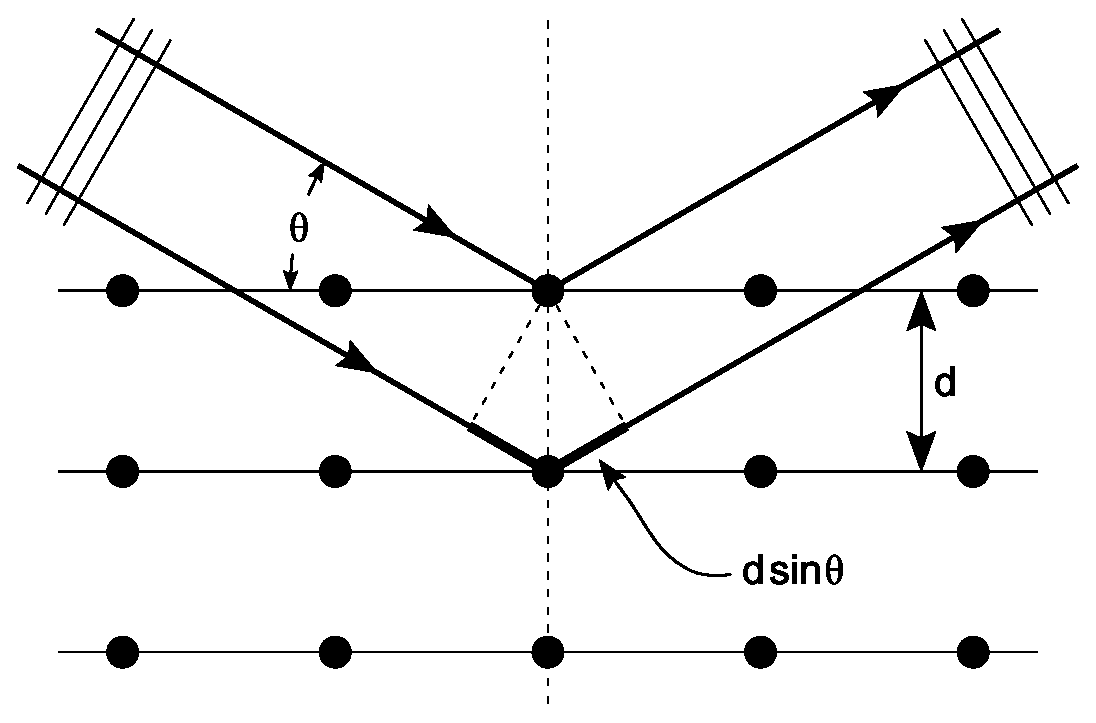
\includegraphics[width=1.5in]{/home/noel/Pictures/Presentations/Insulin/XRay_Braggs_diffraction}
        \end{figure}
        {\tiny Licensed under CC BY-SA 3.0 via Commons \\ https://commons.wikimedia.org/wiki/File:Bragg\_diffraction\_2.svg}
      \end{column}
      \begin{column}{0.5\textwidth}
        \begin{figure}
           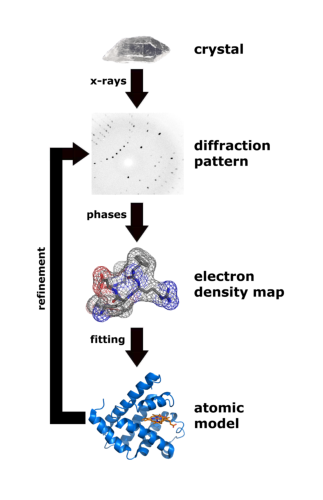
\includegraphics[width=1.5in]{/home/noel/Pictures/Presentations/Insulin/X_ray_diffraction}
        \end{figure}
        {\tiny Licensed under CC BY-SA 3.0 via Commons \\ https://commons.wikimedia.org/wiki/File:X\_ray\_diffraction.png}
      \end{column}
   \end{columns}
\end{frame}
%%%%%%%%%%%%%%%%%%%%%%%%%%%%%%%%%%%%%%%%%%%%%%%%%%%%%%%%%%%%%%%%%%%
\begin{frame}[shrink=10]{Some Powerful Tools Needed for Protein Modeling }
       \begin{enumerate}
             \item Learn some basic Linux command line (see cheat sheet). Work with the Bash shell. It will empower you to do extremely 
                   complicated tasks you never thought you could.
             \item You can use a text editor of your choice to create and save a list of bash commands. This will allow you to generate
                   long lists of complicated procedures needed for protein modeling that you do not have to memorize.
             \item I can help you with the Vi text editor for which I have included a cheat sheet, but the choice of editor is yours.
             \item Learn the basics of git and open a github.com account. This is how you get my code a.k.a Entropy Maxima. This code
                   works with a command line interface.
       \end{enumerate}
\end{frame}
%%%%%%%%%%%%%%%%%%%%%%%%%%%%%%%%%%%%%%%%%%%%%%%%%%%%%%%%%%%%%%%%%%%
\begin{frame}[shrink=15]{Get the code using Git from github.com}
       \begin{enumerate}
             \item Create an account on github.com, and go to https://github.com/noelcjr/EntropyMaxima
             \item Fork the repository on github.com https://guides.github.com/activities/forking/
             \item For the time being you will only use git and github.com to get the code and use it.
                   We will learn how to make changes to the code later. This first lecture is only a demo. 
             \item Now that you have a forked repository in your github account, let's download it to a directory
                   in your computer and use the code in it to modify proteins. 
             \item git clone https://github.com/$<$url to your forked repository$>$/EntropyMaxima
             \item get the files for this lecture: git clone https://github.com/noelcjr/$<$ProteinModelingClass$>$
                   This repository has bash scripts, but do not run them in this folder, just copy the scripts to another folder.
       \end{enumerate}
\end{frame}
%%%%%%%%%%%%%%%%%%%%%%%%%%%%%%%%%%%%%%%%%%%%%%%%%%%%%%%%%%%%%%%%%%%
\begin{frame}[shrink=15]{Explore and Prepare a Protein Structure with Entropy Maxima}
       \begin{enumerate}
             \item Create a folder called Lecture\_1 in the same folder with EntropyMaxima and $<$ProteinModelingClass$>$. 
             \item Type the bash commands: 'mkdir Lecture\_1' and 'cd Lecture\_1'
             \item Copy the Lab\_1\_complete\_structure.sh from the CCL\_lectures repository to the folder just created.
             \item Open Lab\_1\_complete\_structure.sh and run each line at the time.
       \end{enumerate}
\end{frame}
%%%%%%%%%%%%%%%%%%%%%%%%%%%%%%%%%%%%%%%%%%%%%%%%%%%%%%%%%%%%%%%%%%%

\begin{frame}{}
   \begin{center}
   \textcolor{cyan}{\large Thank you}
   \end{center}
\end{frame}
\end{document}
